
% ***************************************************
% Example of an internal chapter
% ***************************************************
%This is an internal chapter of the thesis.
%If you have a long title, you can supply an abbreviated version to print in the Table of Contents using the optional argument to the \chapter command.
\chapter[Results]{Results}
\label{Chap:label}	%CREATE YOUR OWN LABEL.
\pagestyle{headings}

This chapter aims to demonstrate the practicality and efficacy of the designed hardware. Performance metrics such as latency, resource utilisation, timing, and power consumption are analysed to gauge the design's effectiveness. The design is also tested with a small sample of real life packets of different properties to ensure the packet filter can correctly block unwanted packets. Preexisting solutions are then compared with the design, providing insight into the design's relative strength and weaknesses in areas of latency, power and thermal performance.



\section{Latency Performance}

Reducing the latency of hardware packet filtering in embedded systems is one of the key objectives of this thesis. As such, verification of the latency added due to the filtering is essential.

\subsection{Theoretical analysis}
The design employs a 200-stage shift register to temporarily store the incoming packet with each stage being 2bits wide. Given a clock frequency of 50Mhz, the added latency can be calculated to be $200 \times \frac{1}{50\times 10^6} = 4 \times 10^{-6} = 4\mu s$.

\subsection{Measured analysis}


The packet classifier's performance was measured with an Agilent MSO6054A MSO due to its high sampling rate of 4GSa/s. A PMOD pin was connected to output of an xor operation between the carrier sense line (crs\_dv) from the PHY and the crs\_dv post packet filtering. 

This process allowed the added latency to be measured characterised by the time between the rising and falling edge of either pulse as shown in figure \ref{fig:pf_added_latency}. The measured output can be seen to match the theoretical calculation of $4\mu s$.


\begin{figure}[h!]
    \centering
    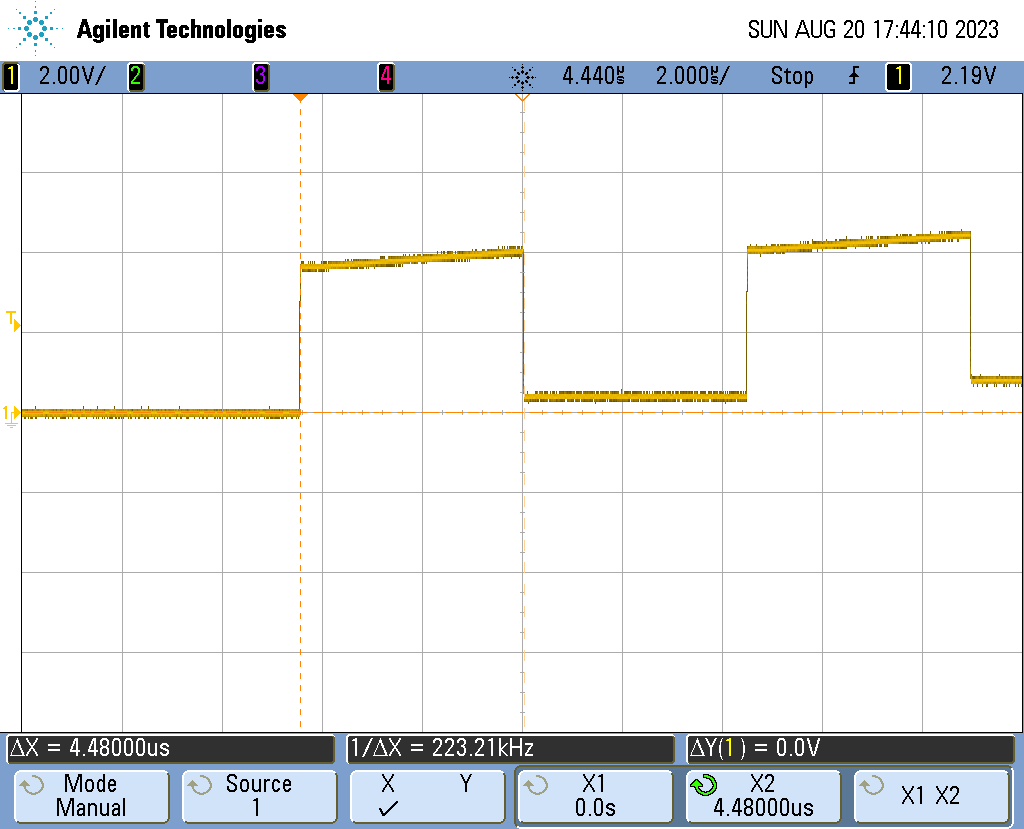
\includegraphics[width=0.75\textwidth]{Images/scope_4.png}
    \caption[Added latency by packet filter waveform]{Added latency by packet filter waveform.}
    \label{fig:pf_added_latency}
\end{figure}


The two distinct pulses are a result of the phase shift between the PHY crs\_dv and the delayed crs\_dv line. Additionally, the distance between the two pulses indicates the size of the packet. 


\subsection{Improvements}
A potential improvement on the design could be to integrate the packet classifier with the Ethernet MAC. This could reduce the added latency to zero by removing the need to store the packet in the additional shift register. The approach would involve storing the incoming packet and if the packet is later deemed to be blocked, the controlling FSM could be reset to ignore the packet. 











\section{Utilisation}

Resource utilisation is an integral part in validating the feasibility of implementing the design on a particular FPGA or microchip. This section details the post synthesis resource utilisation of the design on the Nexys A7-100T FPGA using Xilinx Vivado 2022.2. Namely, the NEORV32, Ethernet hardware and packet filter are analysed.


The resource breakdown referred to in this section can be found in figure \ref{fig:resource_util} while a more detailed breakdown of the resource utilisation including the primitives can be found in appendix \ref{app:res_usage}. 

\begin{figure}[h]
    \centering
    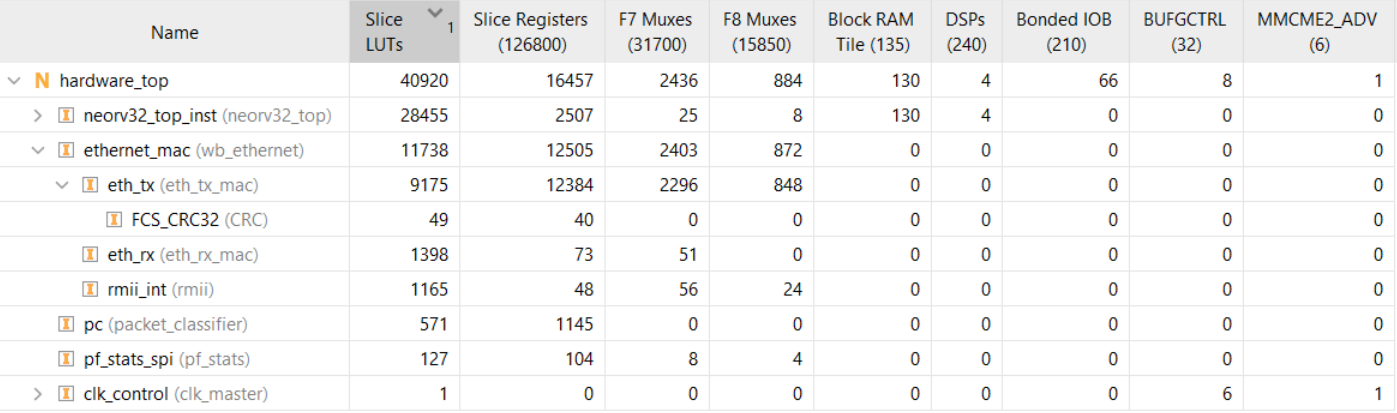
\includegraphics[width=1\textwidth]{Images/FPGAUtilisationResources.png}
    \caption[Summary of the resource utilisation on XC7A100T FPGA]{Summary of the resource utilisation on XC7A100T FPGA.}
    \label{fig:resource_util}
\end{figure}

 
The design as a whole uses a total of 64.5\% of the available slice LUTs, 12.9\% of the available flip flops and 96.3\% of the available BRAM.




\subsection{NEORV32 processor}

significant LUT usage was attributed to the 32-bit wide wishbone interface. Considerable LUT consumption relates to frame buffers used in Ethernet hardware, elucidated further in subsection \ref{sec:eth_hardware_util}.


The NEORV32 SoC consumed the majority (69.5\%, or 28455), of the slice LUTs in the design. While many interfaces were enabled such as SPI, UART, GPIO, external interupts (XIRQ) and the true random number generator, a considerable amount of the LUTs were consumed by the 32bit wide wishbone interface. More specifically, 25992 slice LUTs, or 91.3\% of the NEORV32 usage. 

The large LUT utilisation relates to the frame buffers used in the Ethernet hardware, elucidated further in section \ref{sec:eth_hardware_util}. 

DSP48 blocks were also used by the SoC to handle the multiply operations to free up LUTs. 

The instruction memory (IMEM) and data memory (DMEM) sizes were configured to optimise the remaining BRAM blocks for increasing flexibility in firmware. Specifically, IMEM was allocated 256KB while the DMEM (acting as RAM) amounting to 168KB. 





\subsection{Ethernet hardware}
\label{sec:eth_hardware_util}


Comparatively, the Ethernet hardware accounted for 11738 slice LUTs and 12505 slice registers, most of which is consumed by the transmit logic (78\% LUT and 99\% registers). The considerable LUT utilisation in the transmit logic and NEORV32 Wishbone interface is due to the manner in which the frame buffer is written to. The complex operations such as address validation and array modification for writing to the frame buffer can be seen in listing \ref{lst:code_snippet}. Notably, the address validation specifically implements a 32bit wide comparator and the need to write/modify to the frame buffer array causes large LUT utilisation.

\begin{lstlisting}[style=vhdl, caption={Code for writing to the frame buffer}, label=lst:code_snippet]
if wb_i_addr >= x"13371004" and wb_i_addr <= x"13376410" then         
    -- Subtract 4100 from the address to get the virtual address
    virtAddr := to_integer((unsigned(wb_i_addr(15 downto 0)) - 4100));
    FRAME_BUFFER(8 + virtAddr) := wb_i_dat(31 downto 24);
    FRAME_BUFFER(9 + virtAddr) := wb_i_dat(23 downto 16);
    FRAME_BUFFER(10 + virtAddr) := wb_i_dat(15 downto 8);
    FRAME_BUFFER(11 + virtAddr) := wb_i_dat(7 downto 0);
end if;
\end{lstlisting}

This design choice also influenced the critical path delay as detailed further in section \ref{sec:timing_summary}. Optimisations to this area would be imperative to drastically reduce the resource consumption and improve the critical path delay.

By contrast, the receive logic consumed far less resources of 12\% of the Ethernet MAC's LUTs and only 1\% of the registers. This is attributed to the simpler design which stores the incoming packets with the correct endianness in the frame buffer before subsequently triggering an interrupt upon the packet's arrival. 

The rmii\_init logic acts as the glue logic between the PHY and the MAC. It facilitates the clock and bus domain crossings between the 8bit wide 80Mhz MAC and the 2bit wide 50Mhz RMII PHY. 



\subsection{Packet filter}

The packet classifier consumed a total of 571 slice LUTs and 1145 slice registers, suggesting a potential to increase the number of rules. Though, the fan-in and fan-out will likely need to be considered due to the nature of the implementation. The synthesiser's decision to use registers over BRAM for rule storage is likely due to the rules being small in size and that the BRAM blocks are better used elsewhere.

Alternatively, the minimal resource utilisation indicates that the design is suitable for implementation on smaller FPGAs or ASIC designs and will have negligible impact on the overall silicon area.





\section{Timing Summary}
\label{sec:timing_summary}


Timing analysis of the design provides insight into the critical path delay and the maximum frequency of the design. Basic results are presented in this section and are primarily around the Wishbone interface due to its role in the critical path. Importantly, the Wishbone interface operates at the same clock frequency as the NEORV32 processor which directly impacts the speed of the CPU for software based operations.

Initially, a single 50Mhz clock sourced from the onboard MMCM was used. A post-synthesis analysis indicated a positive slack in the design, allowing for the clock frequency to be updated to 80Mhz. This was done to increase the performance of the CPU so that it could process network packets faster in software.

After resynthesising, a worst negative slack for setup time of -2.634ns was reported with a total of 82 endpoints failing the constraints. Additionally, a worst hold slack of -0.021ns was reported. The identified critical path originates from the Wishbone interface to the BRAM block within the Ethernet hardware, shown in figure \ref{fig:crit_path}. Due to the NEORV32's implementation of the Wishbone bus, the critical path cannot be easily improved and is the leading limitation in the speed of the design. 


\begin{figure}[h]
    \centering
    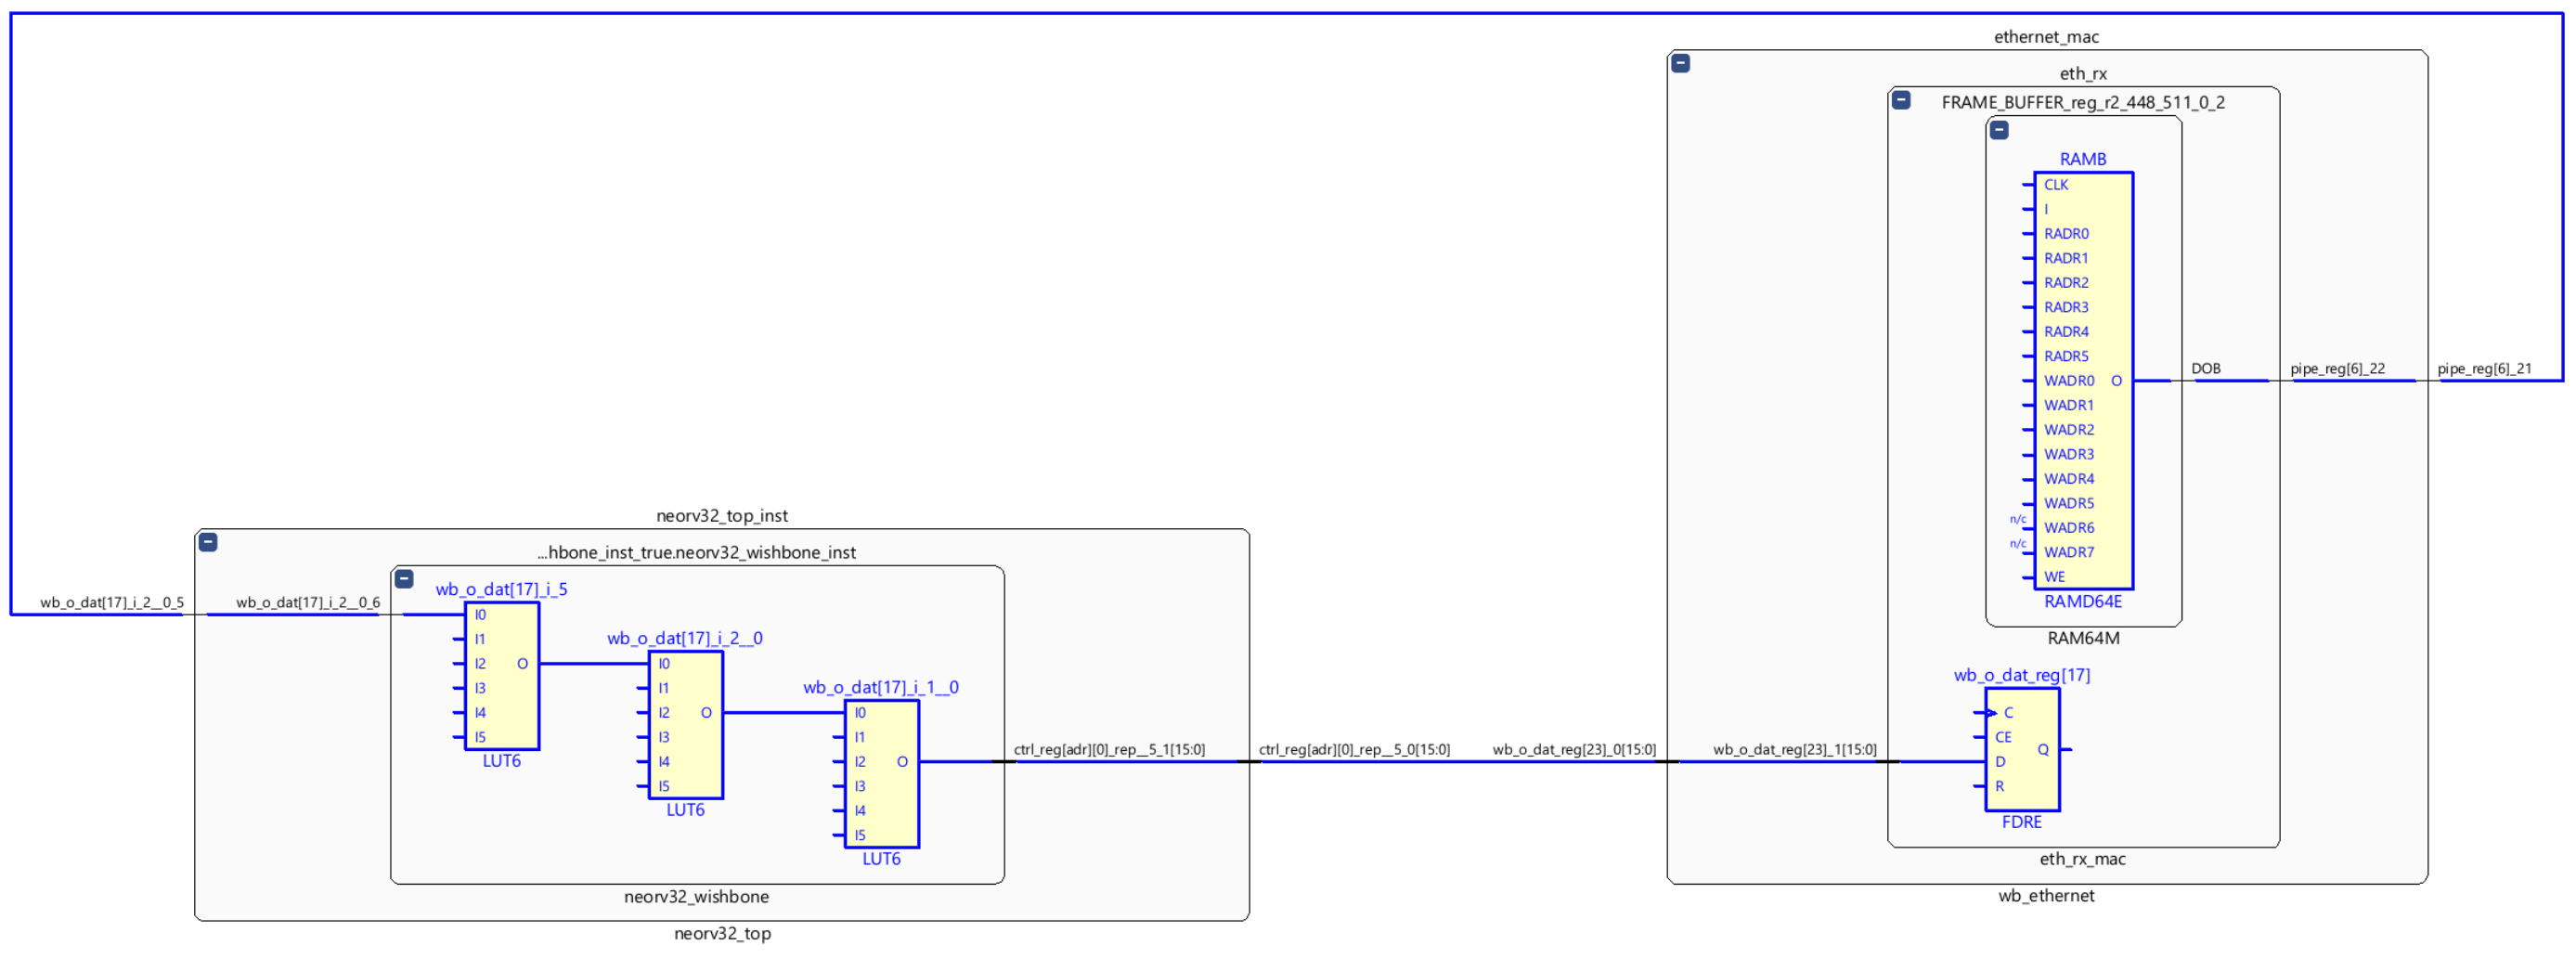
\includegraphics[width=1\textwidth]{Images/critical_path_delay_schematic.png}
    \caption[Critical path in SoC design]{Critical path in SoC design.}
    \label{fig:crit_path}
\end{figure}


While in practice these timing constraints do not crucially impact the design's operation, caution is advised in future adaptations or usage. Other paths were also encroaching on a slack of zero and hence the design was limited to 80Mhz. Testing at 90Mhz was conducted, however, the design was found to be unstable and had a large increase in the number of failing endpoints.

More accurate timing constraints would need to be set to acquire the absolute maximum frequency of the design. Though, this was outside the scope of this thesis. 





















\section{Filtering performance}

Blocking unwanted packets is imperative to a firewall's operation with any packets bypassing the filter rendering it useless. Testing all possible permutations of bits going through the firewall is infeasible due to the shear number of packets needed which is on the order of $2^104$. Instead, a small sample of packets were tested to ensure the filter is working as intended.

\subsection{Test setup}

Four nodes across two networks were tested and the network diagram can be seen in figure \ref{fig:network_layout_test}. The network consisted of three Raspberry Pi 4s and an x86 based Ubuntu machine. 



\begin{figure}[h]
    \centering
    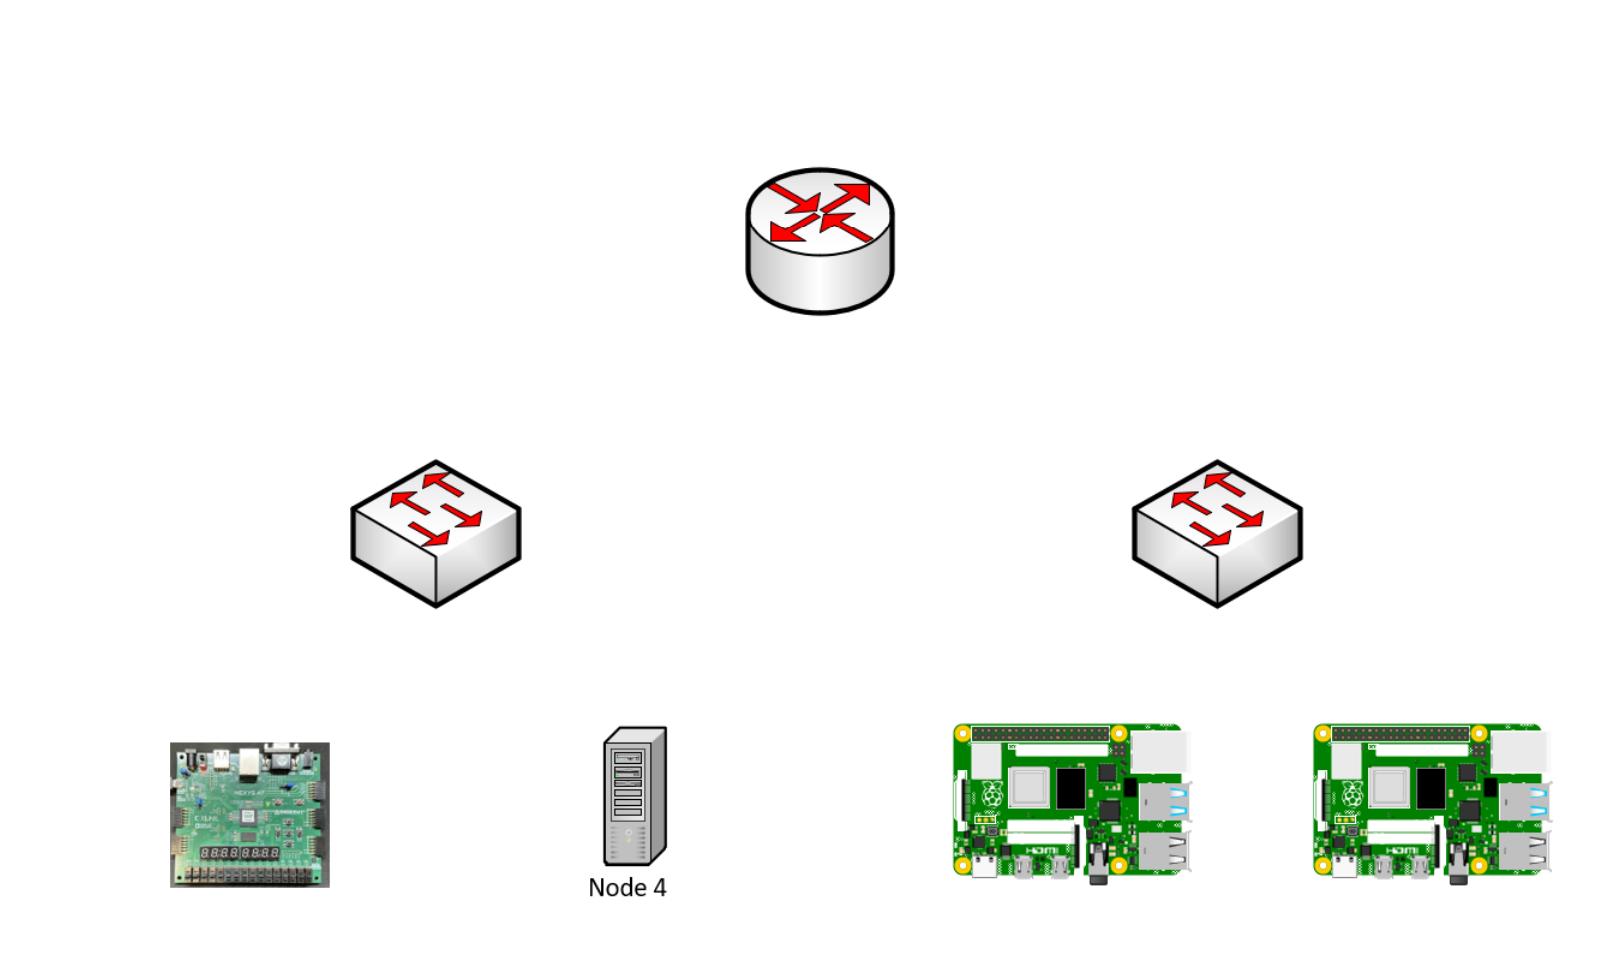
\includegraphics[width=1\textwidth]{Images/NetworkArchitecture.png}
    \caption[Network architecture for firewall tests]{Network architecture for firewall tests.}
    \label{fig:network_layout_test}
\end{figure}

All devices used a common script\footnote[1]{The python \textit{test} script can be found at https://github.com/matty0005/thesis-tools} to test each of the services available on different ports and protocols. 

\begin{table}[h!]
    \centering
    \caption{Firewall configuration for testing}
    \label{tab:firewall_testing_config}
    \begin{tabular}{ccccc}
        \toprule
        Source IP & Destination IP & Source Port & Destination Port & Protocol \\
        \midrule
        any       & 10.20.1.34      & n/a         & n/a              & ICMP     \\
        10.0.0.5  & 10.20.1.34      & any         & any              & UDP      \\
        10.0.0.5  & 10.20.1.34      & any         & 80               & TCP      \\
        10.0.0.93 & 10.20.1.34      & any         & 1337             & TCP      \\
        10.0.0.93 & 10.20.1.34      & any         & 9999             & UDP      \\
        10.20.1.10& 10.20.1.34      & any         & 1337             & any      \\
        10.20.1.10& 10.20.1.34      & any         & any              & UDP      \\
        10.20.1.11& 10.20.1.34      & any         & 9999             & UDP      \\
        \bottomrule
    \end{tabular}
    
\end{table}




\begin{table}[h]
    \centering
    \caption{Firewall Test Cases}
    \label{tab:firewall_test_cases}
    \begin{tabular}{m{2.25cm}m{2cm}m{1.5cm}m{2cm}m{2cm}m{2cm}m{2cm}}
        \toprule
        Device & Dest. IP & Protocol & Src. Port & Dest. Port & Expected Outcome & Actual Outcome \\
        \midrule
        \parbox[c]{2.25cm}{\centering Node1\\\textcolor{gray}{(10.20.1.10)} \vspace*{14pt}} & 10.20.1.34 & TCP & Any & 1337 & Allow & Allowed \\
        \parbox[c]{2.25cm}{\centering Node2\\\textcolor{gray}{(10.20.1.11)} \vspace*{14pt}} & 10.20.1.34 & ICMP & - & - & Allow & Allowed \\
        \parbox[c]{2.25cm}{\centering Node3\\\textcolor{gray}{(10.0.0.5)} \vspace*{14pt}} & 10.20.1.34 & UDP & Any & 9999 & Allow & Allowed \\
        \parbox[c]{2.25cm}{\centering Node4\\\textcolor{gray}{(10.0.0.93)} \vspace*{14pt}} & 10.20.1.34 & TCP & Any & 1337 & Allow & Allowed \\
        \parbox[c]{2.25cm}{\centering Node1\\\textcolor{gray}{(10.20.1.10)} \vspace*{14pt}} & 10.20.1.34 & UDP & Any & 1337 & Allow & Allowed \\
        \parbox[c]{2.25cm}{\centering Node3\\\textcolor{gray}{(10.0.0.5)} \vspace*{14pt}} & 10.20.1.34 & TCP & Any & 80 & Allow & Allowed \\
        \parbox[c]{2.25cm}{\centering Node3\\\textcolor{gray}{(10.0.0.5)} \vspace*{14pt}} & 10.20.1.34 & TCP & Any & 1337 & Deny & Denied \\
        \parbox[c]{2.25cm}{\centering Node2\\\textcolor{gray}{(10.20.1.11)} \vspace*{14pt}} & 10.20.1.34 & TCP & Any & 1337 & Deny & Denied \\
        \parbox[c]{2.25cm}{\centering Node4\\\textcolor{gray}{(10.0.0.93)} \vspace*{14pt}} & 10.20.1.34 & UDP & Any & 1337 & Deny & Denied \\
        \parbox[c]{2.25cm}{\centering Node4\\\textcolor{gray}{(10.0.0.93)} \vspace*{14pt}} & 10.20.1.34 & TCP & Any & 80 & Deny & Denied \\
        \bottomrule
    \end{tabular}
    
\end{table}


The output of the simple test script can be found in appendix \ref{app:testing_pf} for more test cases across all four nodes.





\section{Comparison to preexisting solutions}

To ensure the effectiveness of the designed hardware, some comparisons to preexisting solutions have been made. Three other devices that featured Ethernet connectivity were compared. These devices were the WIZ5500 Pico \footnote[1]{See: https://www.wiznet.io/product-item/w5500-evb-pico/}, Nucloe-F767ZI \footnote[2]{See: https://www.st.com/en/evaluation-tools/nucleo-f767zi.html} and MilkV-Duo \footnote[3]{See: https://milkv.io/duo}. The WIZ5500 pico board uses a Raspberry Pi RP2040 as the MCU at 133Mhz, while it uses the WIZ5500 IC for handling the Ethernet traffic. The WIZ5500 handles layers 1 to 4 onboard and is interfaced over SPI. The Nucleo-F767ZI (referred to as just F767ZI) is powered by the STM32F767 MCU and features an onboard LAN8742A PHY chip onboard. Like the Nexys board, it is also connected over an RMII interface. The STM32 has hardware support for the RMII interface. Finally, the MilkV-Duo is the most recent RISC-V based board which features the CVITEK CV1800B processor. The CV1800B is a 64bit RISC-V processor that operates at a 1Ghz, includes 64MB of RAM and provides the MAC and PHY inside the chip itself.

\subsection{Latency tests}


The same setup was used to test the preexisting solution, except this time GPIO pins were set high and low. It is assumed that the latency of setting the pin high cancels out with the latency of setting the pin low. 




To see how these boards compare in a standard use case, a small program was made to first receive a UDP packet on port 9999 and then reply with another UDP packet. The round trip time was then averaged over 1,000 transactions and has been presented in figure \ref{fig:avg_udp_rtt}. Two tests were conducted, one with a smaller 7 byte payload and another with a larger 256 byte payload to see the effects on packet length had on the round trip time. 

\begin{figure}[ht]
    \centering
    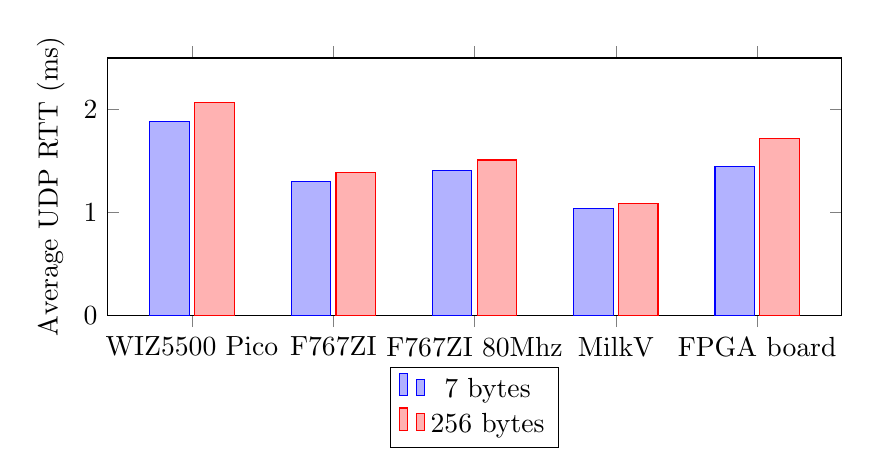
\begin{tikzpicture}
    \begin{axis}[
        ybar,
        symbolic x coords={WIZ5500 Pico, F767ZI, F767ZI 80Mhz, MilkV,  FPGA board},
        xtick=data,
        ylabel={Average UDP RTT (ms)},
        legend style={at={(0.5,-0.2)},anchor=north},
        enlarge x limits=0.15,
        ymin=0,
        ymax=2.5,
        width=0.9\textwidth,
        height=0.4\textwidth,
        bar width=0.5cm
    ]
    \addplot coordinates {
        (WIZ5500 Pico,1.88)
        (F767ZI 80Mhz,1.41)
        (F767ZI,1.30)
        (FPGA board,1.45)
        (MilkV,1.04)
    };
    \addplot coordinates {
        (WIZ5500 Pico,2.07)
        (F767ZI 80Mhz,1.51)
        (F767ZI,1.39)
        (FPGA board,1.72)
        (MilkV,1.09)
    };
    \legend{7 bytes,256 bytes}
    \end{axis}
    \end{tikzpicture}
    \caption{Average UDP RTT for different devices and payload sizes.}
    \label{fig:avg_udp_rtt}
    \end{figure}
    
A table of the results can be found in appendix \ref{app:udp_ping_measurements}.

The larger difference in the round trip times for the FPGA board over the others indicates that the processor is taking longer time to process the packet in software as the time difference on receiving the packet is $\frac{249 \times 8}{100 \times 10^6}=19.9\mu s$. This could also be due the FreeRTOS-Plus-TCP stack using more computations per packet than LwIP on the F767ZI. The MilkV not only run's linux, it operates at 12.5 times the frequency, 1Ghz. 

\subsection{Firewall performance}

The hardware packet filter in this design has previously be found to induce a 4.48us delay and does not change the throughput of the device. 

A software based implementation of the firewall was created on the Nucleo-F767ZI board. Also with 8 rules. After measuring with an with an oscilloscope for the time it takes to compute whether or not to forward the packet, the timings depended on first how many rules there are, where a valid rule is matched (start or end of the sequence), if there is like terms between invalid rules and so on. 

As a best case, the time was found to be 3.14us (figure \ref{fig:sw_pf_best_case}) while an average-to-bad case was 10.76us (figure \ref{fig:sw_pf_bad_case}).



\begin{figure}[h]
    \centering
    \begin{subfigure}[b]{0.45\textwidth} % Adjust the width to your needs
        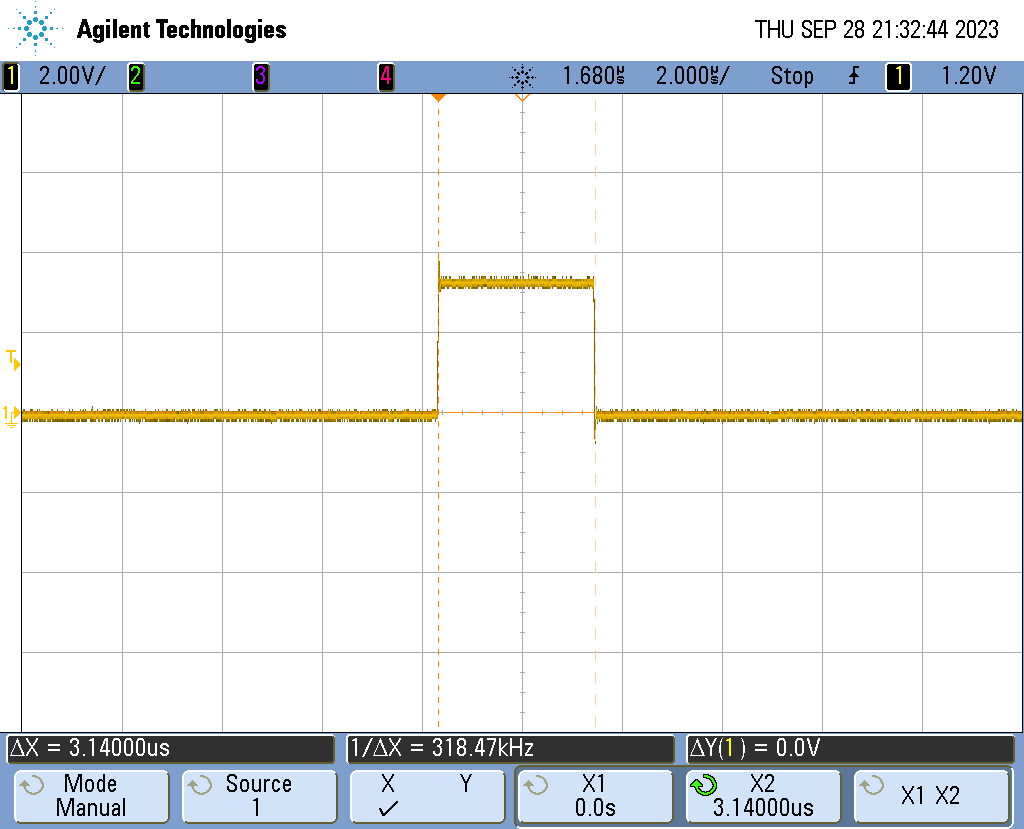
\includegraphics[width=\textwidth]{Images/sw_pf_best_case.png}
        \caption{Best case scenario}
        \label{fig:sw_pf_best_case}
    \end{subfigure}
    \hfill % this will add a small space between the two images
    \begin{subfigure}[b]{0.45\textwidth} % Adjust the width to your needs
        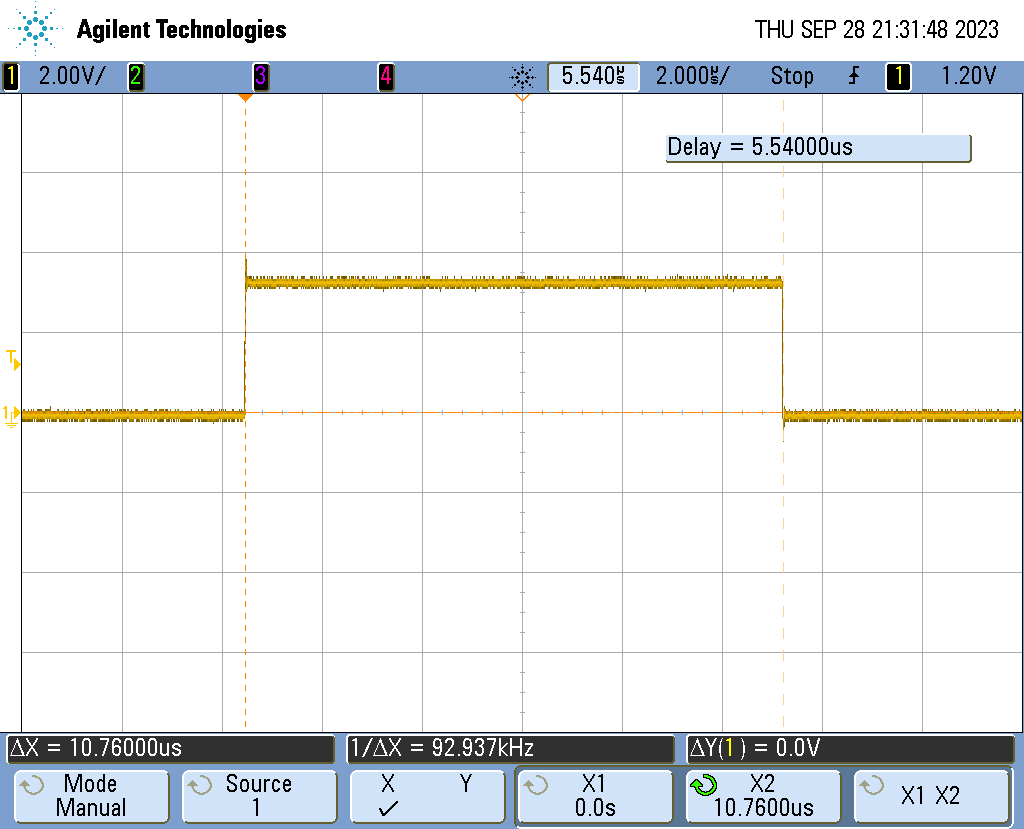
\includegraphics[width=\textwidth]{Images/sw_pf_bad_case.png}
        \caption{Average case}
        \label{fig:sw_pf_bad_case}
    \end{subfigure}
    \caption{Software packet classifier timings}
    \label{fig:sw_pf_timings}
\end{figure}

Importantly these delays unlike the FPGA one, do impact throughput as the processor is limited to filtering the packets and not doing other things like recieving another packet. 

\subsection{Thermal analysis}

A thermal camera was used to record the temperatures periodically. At an ambient room temperature of $24.8\degree C$ throughout the test, after 5mins the WIZ5500 ethernet chip heated to $58.0\degree C$ and RP2040 was at $46.6\degree C$. While the FPGA was at $38.0 \degree C$. This is a bit of an unfair comparison as the physical size of the FPGA is much larger than the WIZ5500. After two hours of constant UDP ping requests to both devices, figure \ref{fig:thermal_2hr_fpga_pico} shows the FPGA board and WIZ5500 board's temperature gradient. The FPGA plateaued to a maximum of $40.4 \degree C$ while the WIZ5500 was $1.c \degree C$ cooler at, $56.8 \degree C$. This could be due to accuracy of the measurements, in addition to not getting aiming the thermal camera in the hottest part. The RP2040 chip however was measured to be $53.2 \degree C$. Some additional thermal images can be found in the appendix. 



\begin{figure}[h]
    \centering
    \begin{subfigure}[b]{0.45\textwidth} % Adjust the width to your needs
        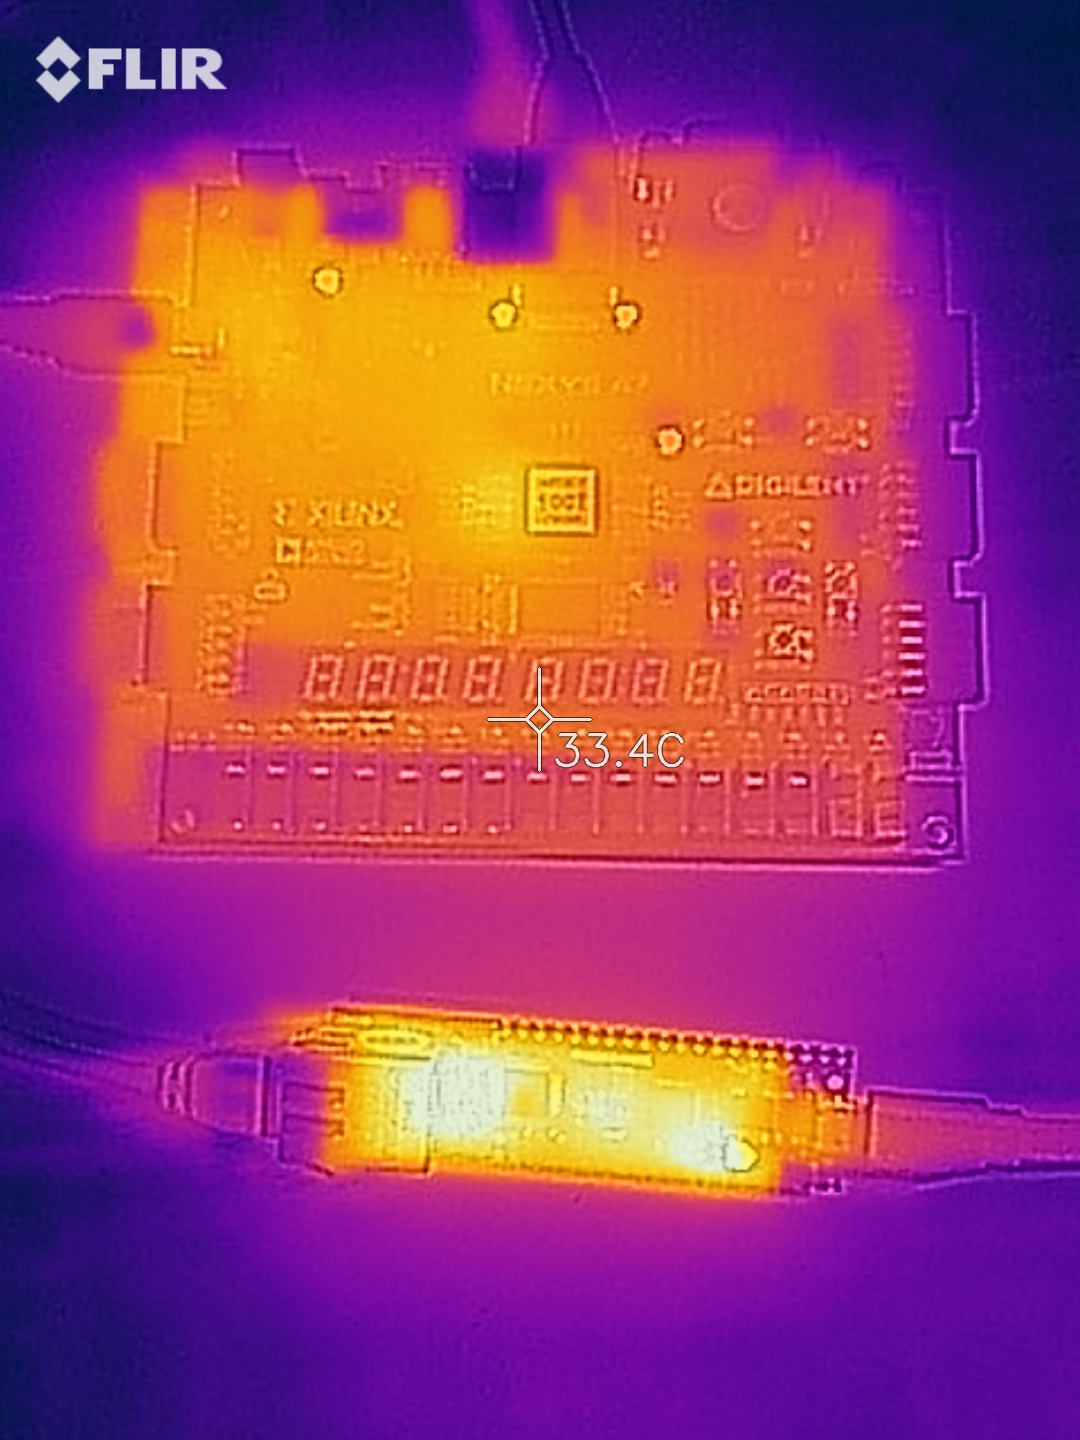
\includegraphics[width=\textwidth]{Images/flir_2hs.jpg}
        \caption{FPGA board (top) and WIZ5500 Pico (bottom)}
        \label{fig:thermal_2hr_fpga_pico}
    \end{subfigure}
    \hfill % this will add a small space between the two images
    \begin{subfigure}[b]{0.45\textwidth} % Adjust the width to your needs
        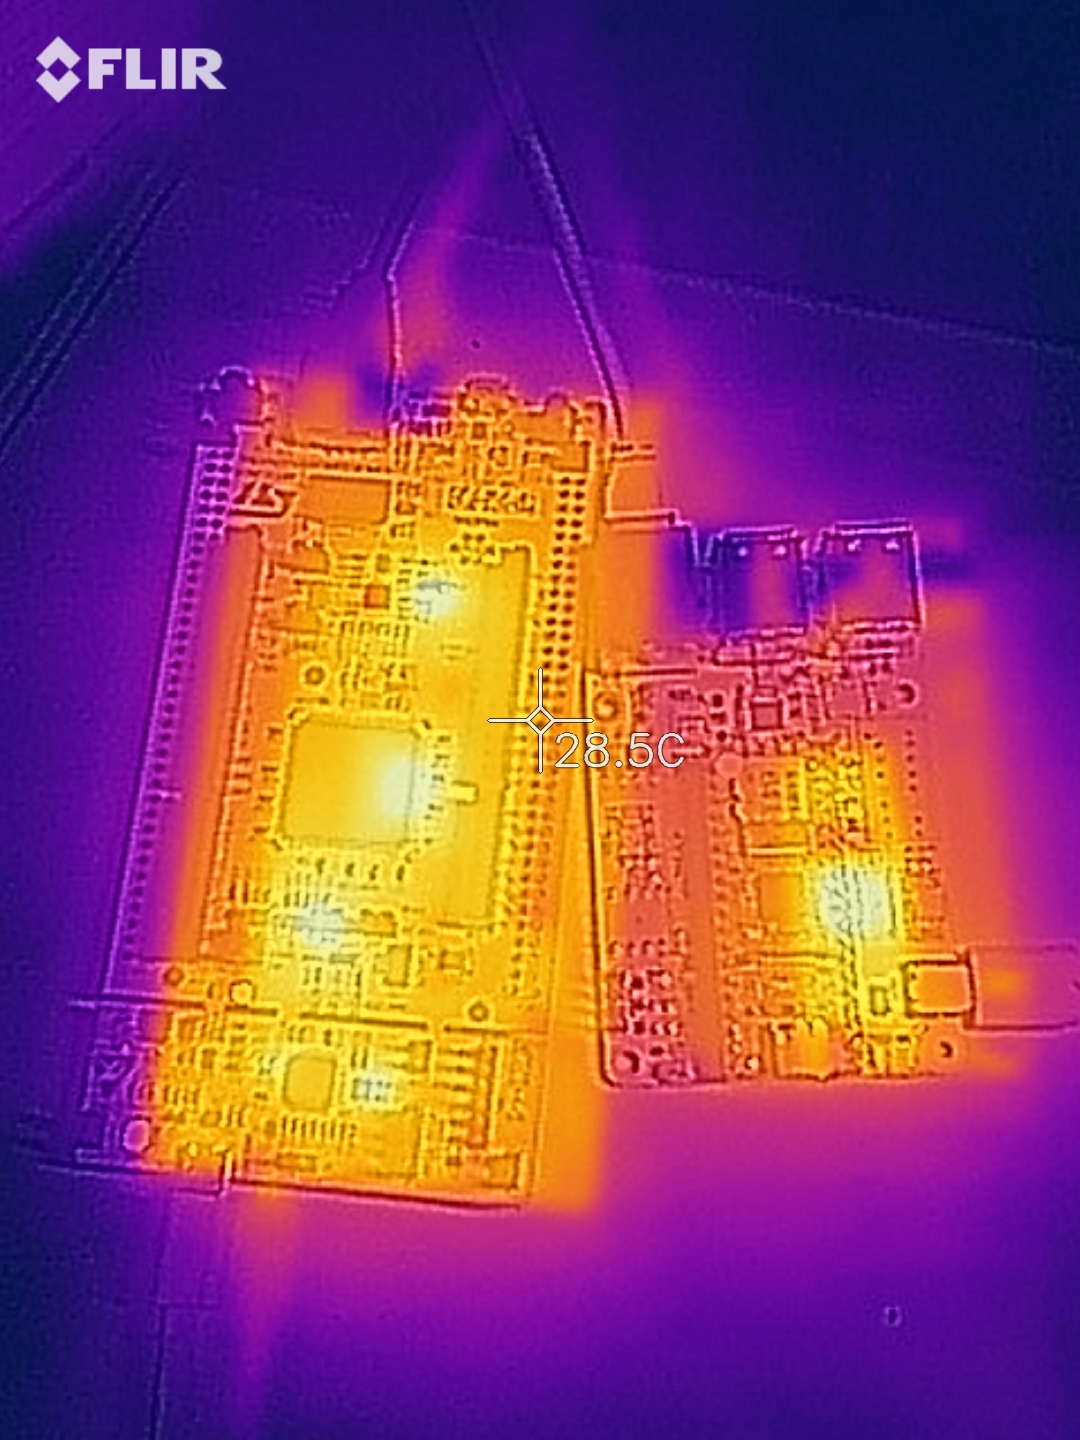
\includegraphics[width=\textwidth]{Images/flir_nucleo_milkv.jpg}
        \caption{Nucleo board (left) and MilkV Duo (right)}
        \label{fig:thermal_2hr_nucleo_milkv}
    \end{subfigure}
    \caption{Thermal images of boards under test after two hours}
    \label{fig:thermal_2hr}
\end{figure}

A STM32 Nucleo-F767ZI board and a MilkV Duo board was also tested (figure \ref{fig:thermal_2hr_nucleo_milkv}). After two hours, the STM32F767 reached a temperature of $36.8\degree C$ while the LAN8742 reached $36.2\degree C$. The MilkV Duo which consists of the Ethernet PHY internally reached $38.1\degree C$ after two hours.

These temperatures though cannot be considered as accurate, but rather used as an indication to see the hotspots in the boards and determine if one board gets excessively hot over the other. With this in mind, The WIZ5500 seems to reach the hottest out of the boards tested. The FPGA itself was consistently the lowest temperature across the board with the MilkV coming in a close second (considering it only has one source of heat).


\subsection{Power consumed between boards}

\begin{figure}[ht]
    \centering
    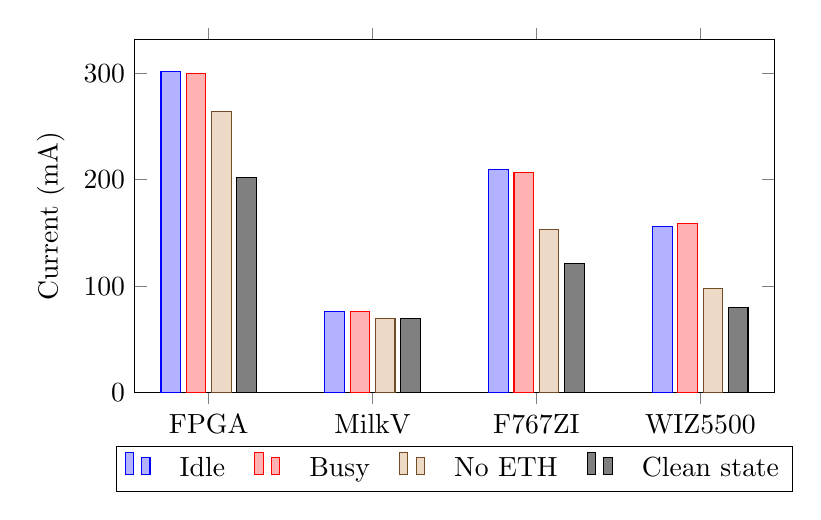
\begin{tikzpicture}
        \begin{axis}[
            ybar,
            bar width=0.25cm,
            width=0.8\textwidth,
            height=0.5\textwidth,
            enlarge x limits=0.15, % Adjusted value to make the bars closer
            ylabel={Current (mA)},
            symbolic x coords={FPGA, MilkV, F767ZI, WIZ5500},
            xtick=data,
            legend style={
                at={(0.5,-0.15)},
                anchor=north,
                legend columns=-1,
                legend cell align=left,
                legend image post style={scale=1}, % Adjust this value for spacing
                column sep=0.3cm % Adjust the space between each legend entry
            },
            legend cell align=left,
            ymin=0,
        ]
        \addplot coordinates {
            (FPGA, 301.4)
            (MilkV, 76.27)
            (F767ZI, 209.25)
            (WIZ5500, 155.88)
        };
        \addlegendentry{Idle}
        
        \addplot coordinates {
            (FPGA, 300.13)
            (MilkV, 76.53)
            (F767ZI, 206.9)
            (WIZ5500, 158.67)
        };
        \addlegendentry{Busy}
    
        \addplot coordinates {
            (FPGA, 264)
            (MilkV, 69.23)
            (F767ZI, 153.46)
            (WIZ5500, 97.9)
        };
        \addlegendentry{No ETH}

        % New data for "Complete Idle"
        \addplot coordinates {
            (FPGA, 202.13)
            (MilkV, 69.23)
            (F767ZI, 121.31)
            (WIZ5500, 80.35)
        };
        \addlegendentry{Clean state}

        \end{axis}
    \end{tikzpicture}
    \caption{Comparison of Idle, Busy, and No eth currents for devices}
    \label{fig:power_comparison}
    \end{figure}
    


In Appendix \ref{app:current_measurements} figure \ref{tab:power_consumption} shows the same data in table form presenting numerical values.

From figure \ref{fig:power_comparison}, the difference between the clean state and the busy states can be learned. The FPGA board had the largest difference at 99.27mA, compared to the 87.94mA difference witnessed in the F767ZI board. What must be taken into consideration is that the measurement for the FPGA board is without the hardware design (both Ethernet MAC, packet filter and RISC-V core) applied. Another reading of 283.75mA was observed when the design and hardware had been loaded (no firmware). What this means is that even though the FPGA board has the highest quiescent current amoungst the devices, it still has the larger design current for the project itself. 

The smaller difference from the no Ethernet attached to the active state on the FPGA in comparison to the differences noticed on the F767ZI and WIZ5500 boards indicates that this is likely due to the MAC hardware in the F767ZI and WIZ5500 enters a sleep state to consume less current. The hardware designed in this thesis did not take this case into consideration. 


\subsection{Security analysis}
Only the FPGA board designed in this thesis has a hardware packet filter. The other devices need to implement a software based packet filter. On the surface this makes the two sound equivalent. However, software based firewalls may be susceptible to power-glitch attacks. Power glitch attacks are a common vulnerability in embedded systems. It consists of switching off and on power very rapidly at a critical point in the code to essentially bypass a certain instruction. While this is highly unlikely and often hard to implement, it is an advantage nonetheless.  

As the packet filter is designed in hardware and is directly reading the bits from the PHY and doesn't consist of instructions as such, the hardware packet classifier in this design should not susceptible to a power glitch attack. Formal testing of this however was not part of the scope of this thesis.


\section{Power analysis}

\subsection{Theoretical analysis }

Vivado provides a post synthesis power analysis summary for the design. While these are depenant on a lot of variables, they should provide a basis as to what to expect and help with optimisation of power within the design. The design was observed to take a total of 0.487W (figure \ref{fig:post_synth_power_summary}) where 0.383W of that is dynamic and depends on the operations taking place. 

\begin{figure}[h]
    \centering
    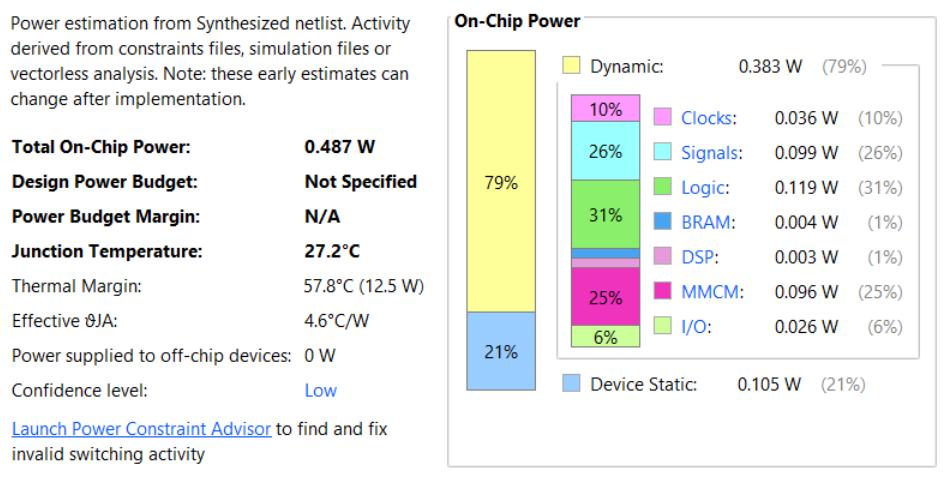
\includegraphics[width=0.75\textwidth]{Images/power_summary.png}
    \caption[Post synthesis power summary for design]{Post synthesis power summary for design.}
    \label{fig:post_synth_power_summary}
\end{figure}


Vivado further breaks down the design into the different hierarchical components shown in table \ref{tab:power_consumption}. Notably most of the power consumption in the design is a result of the RISC-V processor in the design. Notably the Ethernet hardware and packet filter consumes under 100mW. 

\begin{table}
    \centering
    \caption{Power consumption of components.}
    \begin{tabular}{lc}
        \toprule
        Name & Total (W) \\
        \midrule
        neorv32 & 0.158 \\
        clk control & 0.097 \\
        ethernet\_mac & 0.097 \\
        packet classifier & 0.002 \\
        \bottomrule
    \end{tabular}
    \label{tab:power_consumption}
\end{table}






\subsection{Measured analysis}

As the voltage would remain constant between devices (all powered over USB), only the current was measured. These results however should be taken with caution as they do not account for regulator inefficiencies and do not give a true current reading of the device, rather just an indication. 


The device for testing the current was the Nordic Semiconductor Power Profiler Kit 2 which can record at up to 100kSa/s. For the tests in this report, only a sampling rate of 10kSa/s was used as it produces less noisy results. 

As a baseline, the Nexys A7 board draws 200mA (1W at 5V) with no design applied and is due to all the additional components on the board. With the design loaded up but without the processor flashed, the board took 284.4mA. After flashing the board, the idle current reached an average of 301.84mA. Multiplying this by 5V gives us a power draw of 1.51W. To factor in the quiescent current for the other devices on the FPGA board and if it is assumed that the 200mA reading solely for the other components on the FPGA board, it can be found that the design draws around 0.51W. This is rather close to what the synthesis tool calculated. 

A series of tests were then done and the currents were measured. By pinging the device every 50ms, the average current consumption was 300.72mA. Interestingly, the current consumption was cyclic similar to what is shown in figure \ref{fig:ppk_icmp_ping}. A UDP ping test was conducted and had an average current draw of 301.13mA. In both the ICMP and UDP pings, the current consumption was of similar style where the variance of the current was about 10mA. 


If the packets are now blocked by the filter, more about the design in terms of power consumption can be learned. After adding a rule in the packet filter, very little could be observed in the current consumption over the unblocked case. The same cyclic pattern in figure \ref{fig:ppk_icmp_ping} could be seen. An average of 300.92mA was been consumed by the device and is within the margin of error of the device. Figure \ref{fig:ppk_icmp_ping} shows the that the period for the current waveform is about 83ms, which is much larger than the 50ms between pings to the device. After filming the status LED on the PHY output at 240 frames per second, the period of the LED was 20 frames equivalent to $\approx 84ms$ which aligns with the current measurements. 


\begin{figure}[h]
    \centering
    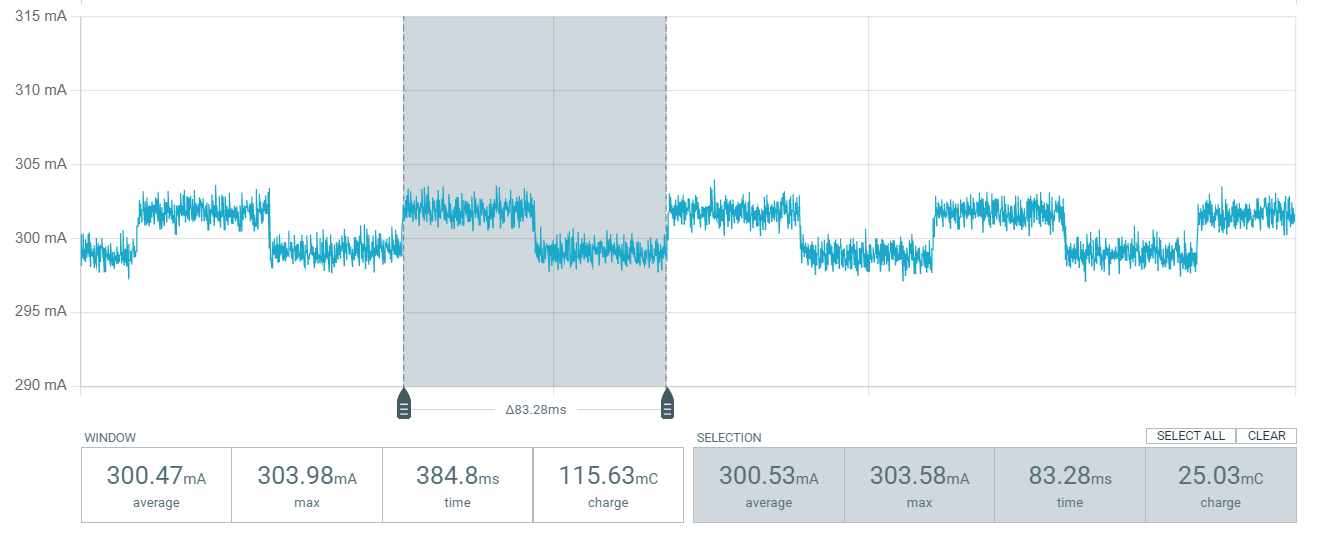
\includegraphics[width=0.9\textwidth]{Images/PPK_ping_zoom.png}
    \caption[Zoomed in current consumption for ICMP pings]{Zoomed in current consumption for ICMP pings.}
    \label{fig:ppk_icmp_ping}
\end{figure}



The next test was done when accessing the webserver. Figure \ref{fig:ppk_http_annotated} shows 5 different regions where each region is a result of a different action. The left most tests is from the inital HTTP requests to get the index page. Notably, there is 2 separate sections here, this is because the client fetches the html, css and favicon first and then requests the main (and much larger) javascript file after. The readings for each of these points is given as: average current, maximum current and time going from top to bottom. 

The second test is what happens when you click to navigate to the about page. The third event is when navigating to the config page and the 4th event is what happens when you press the 'load rules' button. The final test case is a refresh on the main page for the statistics. Notably, as the javascript (thus client) is doing the routing and page handling, future requests to get the contents of the pages are not needed, but only small API requests to update the data. Coincidentally, these first 3 requests also trigger a SD card read and explains the higher current draw. The fourth request also creates a read request to the SD card, but only needs to read a single page. The fifth request does not involve a read or write to the SD card, but rather just a simple SPI transaction takes place and consequently doesn't draw much additional power. 

\begin{figure}[h]
    \centering
    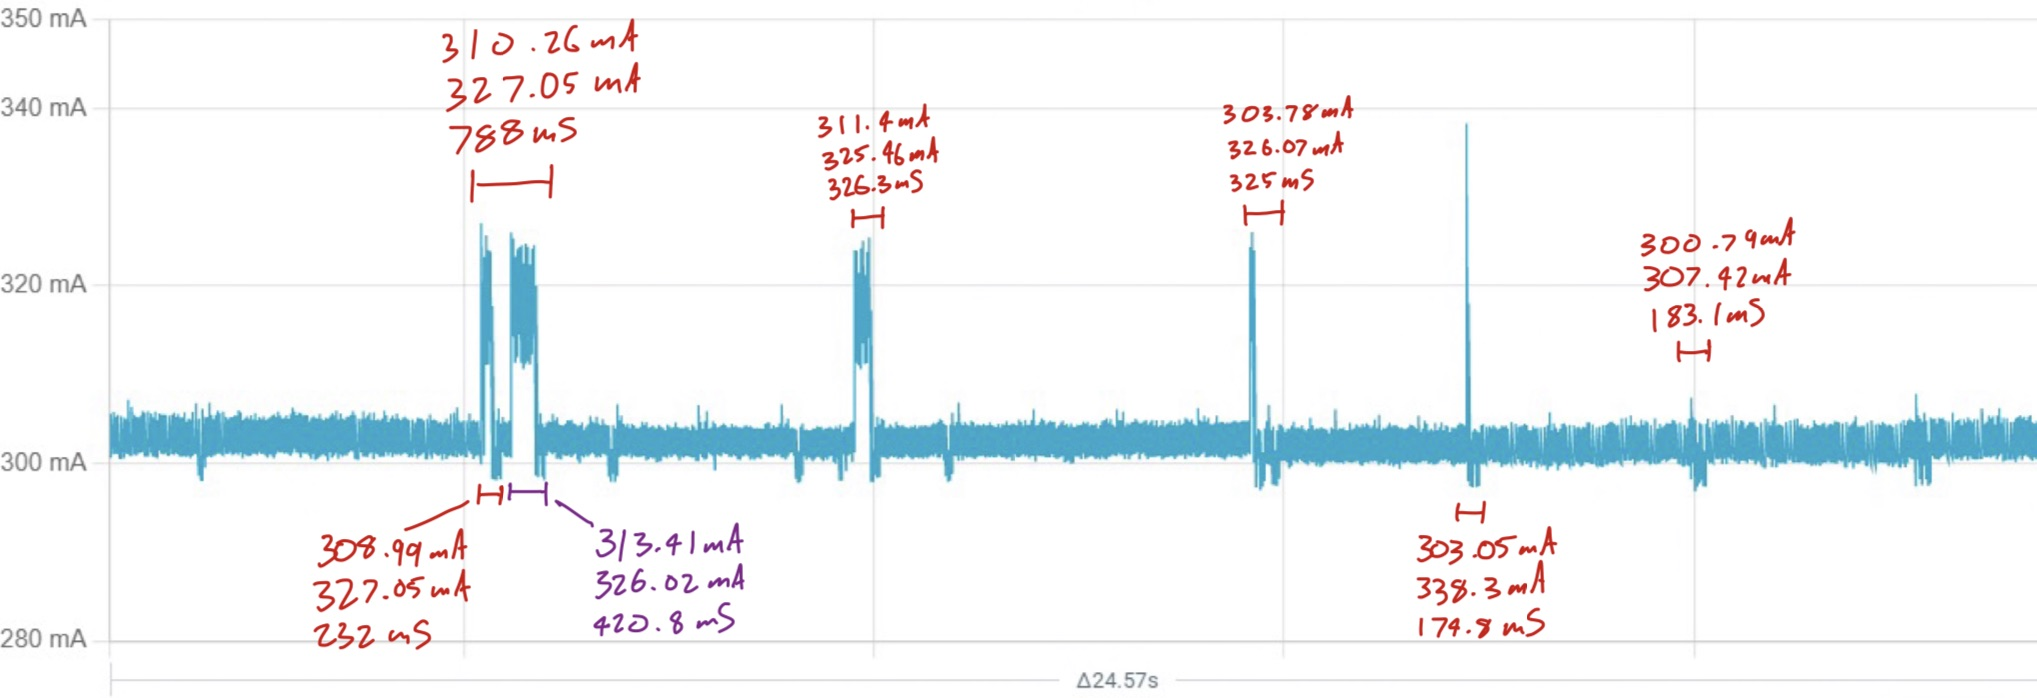
\includegraphics[width=0.9\textwidth]{Images/PPK_http_annotated.png}
    \caption[Current consumption of FPGA board with HTTP requests]{Current consumption of FPGA board with HTTP requests.}
    \label{fig:ppk_http_annotated}
\end{figure}













\section{Modifications}
The design was changed from the 2 ethernet interfaces to a design with just a single ethernet interface. 
\subsection{Limitations}
\subsubsection{PMOD Interface}

There are 5 PMOD connectors on the development board. Initally, one of these would be used for a second Ethernet PHY, but due to bandwidth limitations of the interface, the design had to be altered. The recommended bandwidth of these ports are 25MHz while the Ethernet RMII PHY would have been using 50Mhz signals over the interface. As such, signal integrity issues arose (see figure \ref{fig:eye_diagram}) and restricted the use to just one interface - the onboard PHY. A new development board with two PHYs would be needed.

\begin{figure}[h]
    \centering
    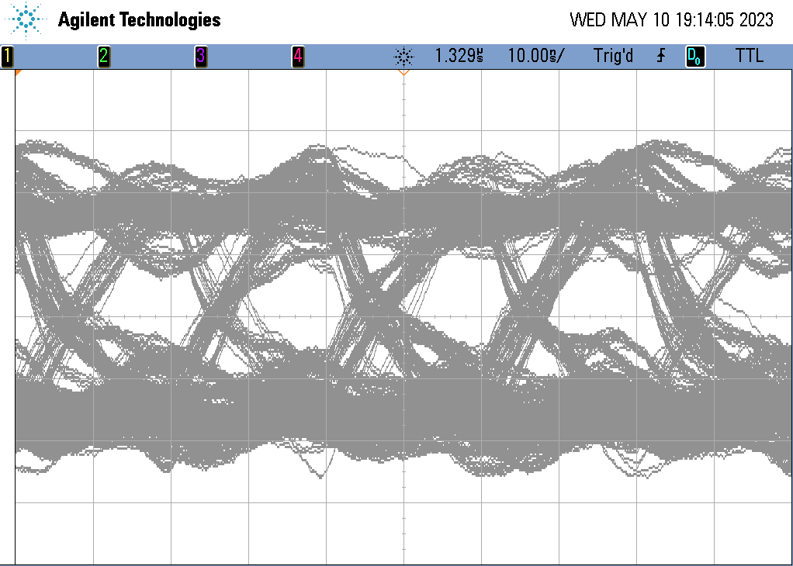
\includegraphics[width=0.65\textwidth]{Images/EyeDiagramTX.png}
    \caption[Eye diagram of TXD through PMOD interface]{Eye diagram of TXD through PMOD interface.}
    \label{fig:eye_diagram}
\end{figure}